\chapter{大规模社交多媒体数据快速处理}
社交多媒体数据由于规模庞大,需要耗费大量的计算资源和时间进行处理。本章主要从特征选取
和模型简化的角度讨论大规模社交多媒体数据的快速处理。

本章首先介绍用于大规模高维数据的特征选取算法。 对于社交多媒体数据的特征描述
不仅包括高层次的卷积神经网络特征,还包含低层次全局特征(如颜色特征,纹理特
征),局部特征(如SIFT,SURF)以及用来通过局部特征描述整体视觉信息的词袋特征等。实际应用
中需要根据需求选取对目标任务最有用的特征子集,这对于大规模社交多媒体数据的处理速度以及
移动设备有限的计算能力和内存空间尤其重要。此外,去除特定任务不相干的特征,还可以提高特
征的表达能力。

其次,本章介绍用于深度卷积神经网络的模型简化算法。
深度卷积神经网络在很多计算机视觉领域都表现出很好的性能,
然而网络的深度和模型参数通常比较大,例如经典的 VGG-16 网络包含超过200M的模型参数。
大量的模型参数意味着在实际应用中需要大量的计算资源和时间,极大地限制了深度神经网络
在大规模图片检索和图片识别等任务上的应用。此外,深度网络在移动设备上的应用已经成为一种
趋势。由于移动设备计算能力的限制,在不影响模型准确度的条件下简化深度网络模型已经成为迫
切的需要。

\section{二阶在线特征选取}
特征选取是指从数据中移除不相关或者冗余特征的过程。在当前大数据的背景下,特征选取
已经成为了十分重要的一项技术,并在多个领域尤其是高维数据的场景下获得了
广泛应用~\cite{Bolon015RAE,Zhai14EBD}。尽管特征选取已经被广泛的研究,大部分的算法
都属于批处理学习。批处理学习的主要问题在于它需要将整个数据集加载到内存中,由于计算机的
内存容量无法跟上数据规模,这对于实际问题中大规模高维数据显然不具有可伸缩性。此外,
批处理方法假设所有的训练数据和特征在训练前已经给定,而实际场景中需要处理的往往是流数据,
并可能伴随有新的特征出现。为了克服已有算法的这些问题,
近年来有部分工作研究在线特征选取~\cite{wang2014online,wu2010online,yang2013efficient}。
在线学习的优点在于算法每次迭代只处理一个数据,从而达到很高的可伸缩性,
并且可以很好地应对数据中模式和特征的变化。然而,目前已有的在线特征选取算法复杂度仍然过高,
模型的准确率与批处理方法也有不小差距。因此,文本提出了二阶在线特征选取算法,不仅对于
大规模高维数据具有很高的可伸缩性和学习效率,算法的准确率也与批处理方法十分接近。

不失一般性,我们首先研究二分类问题,并在~\ref{ssec:smofs}章节将算法扩展到多类问题。
令$\{(\x^t,y^t)|t=1,\ldots, T\}$表示训练过程中依次收到的数据,每个数据$\x^t
\in
\R^d$是一个$d$维的向量,数据类别$y^t\in\{+1,-1\}$。
在线学习算法将学习一个相同维度的分类器$\w \in \R^d$。
在时刻$t$,算法接收到数据$\x^t$,并基于当前的模型参数$\w^t$预测它的类别$\hat{y}\in\{+1,-1\}$。
\begin{equation}\label{eqn:predict}
    \hat{y}^t = \sign(\w^t \cdot \x^t)。
\end{equation}
预测完以后,算法将得到真实的类别$y^t$,从而衡量在数据$(\x^t,y^t)$上的损失函数$\ell(\w^t)$。
损失函数通常为真实类别和预测结果之间的差值的函数。在每轮迭代的最后,算法根据特定的规则更新
模型参数$\w^t$。例如,在线梯度下降算法更新的规则为:
\begin{equation}
    \w^{t+1} = \w^t + \eta^ty^t\x^t,
\end{equation}
$\eta^t$是时刻$t$的学习率(learning
rate)。根据不同的更新规则,在线学习算法可以分为两类:
\begin{itemize}
    \item 一阶算法:本质上是梯度下降算法~\cite{crammer2006online};
    \item 二阶算法:挖掘输入数据的几何特点~\cite{crammer2009adaptive}
        或构建目标方程的近似海森矩阵~\cite{duchi2011adaptive};
\end{itemize}
在线特征选取需要选取权重向量$\w^t$中相对较小的一部分元素,并将其他元素设为$0$。
换句话说,我们对$\w$的$L_0$范式施加如下约束:
\begin{equation}
    \|\w\|_0 \leq B, \|\w\|_0 = \sum_{i=1}^d w_i^0,
\end{equation}
$B$是预先定义的常数,因此,最多只有$\x$的$B$个特征被用来做预测。

\section{置信度加权二阶在线特征选取}
在线特征选取最直接的一种做法是运用截断感知机算法(Perceptron with
Truncation, PET)~\cite{wang2014online}。具体来说,分类器在每次迭代首先
根据$\w^t$预测类别$\hat{y}^t$。如果$\hat{y}^t$是正确的,则$\w^{t+1}=\w^t$;
否则,分类器根据感知机规则更新$\w^t$:$\hat{\w}^{t+1} = \w^t + \eta y^t\x^t$。
更新后的参数进一步被保留绝对值最大的$B$个元素,其他元素的值设为$0$.截断后的分类器参数
$\w^{t+1}$将被用于下一次迭代数据的预测。算法~\ref{alg:pet}显示了PET算法的框架,
算法~\ref{alg:truncate}显示了在线特征选取的截断函数。


\IncMargin{1em}
\begin{algorithm}
\SetKwData{Left}{left}\SetKwData{This}{this}\SetKwData{Up}{up}
\SetKwFunction{Union}{Union}\SetKwFunction{FindCompress}{FindCompress}
\SetKwInOut{Input}{input}\SetKwInOut{Output}{output}

\Input{$B$ - 需要选取的特征个数,$\eta$ - 学习率}
\Output{权重向量$\w^T$}
\BlankLine
初始化$\w^1 = \zero$\;
\For{$i\leftarrow 1$ \KwTo $T$}{
    接收到数据$\x^t\in \R^d$,预测类别$\hat{y}^t = \sign(\w^t\cdot \x^t$\;
    接收真实类别$y^t$\;
    计算损失函数$\ell(\w^t)$\;
    \If{$\ell(\w^t)>0$}{
        $\hat{\w}^{t+1} = \w^t + \eta y^t \x^t$\;
        $\w^{t+1} = \Truncate(\hat{\w}^{t+1},B)$\;
    }
}
\caption{PET:截断感知机算法框架}\label{alg:pet}
\end{algorithm}\DecMargin{1em}

\IncMargin{1em}
\begin{algorithm}
\SetKwData{Left}{left}\SetKwData{This}{this}\SetKwData{Up}{up}
\SetKwFunction{Union}{Union}\SetKwFunction{FindCompress}{FindCompress}
\SetKwInOut{Input}{input}\SetKwInOut{Output}{output}

\Input{$\hat{\w}$ - 权重向量,$B$ - 需要选取的特征个数}
\Output{截断的权重向量$\w$}
\BlankLine
$\w=\hat{\w}$\;
\If{$\|\hat{\w}\|_0 > B$}{
    除了$\w$的绝对值最大的$B$个元素,其他元素全部设为0\;
}
\caption{Truncate: 截断函数}\label{alg:truncate}
\end{algorithm}\DecMargin{1em}

根据Wang等人的分析,上述算法在实际应用中并不总能取得很好的效果。它不能保证被截断
的参数足够小,因而不能保证很小的错误率。因此,他们在截断之前运用稀疏投影,
提出了一阶在线特征提取算法(FOFS)。FOFS算法保证了每轮迭代分类器参数$\w^t$都限制在
一个$L_1$范式约束的超体内部。算法显示了FOFS算法的细节。

\IncMargin{1em}
\begin{algorithm}
\SetKwData{Left}{left}\SetKwData{This}{this}\SetKwData{Up}{up}
\SetKwFunction{Union}{Union}\SetKwFunction{FindCompress}{FindCompress}
\SetKwInOut{Input}{input}\SetKwInOut{Output}{output}

\Input{$B$ - 需要选取的特征个数,$\eta$ - 学习率,$\lambda$ - 正则化参数}
\Output{截断的权重向量$\w$}
\BlankLine
$\tilde{\w}^{t+1} = (1-\lambda\eta)\w^t + \eta y^t \x^t$\;
$\hat{\w}^{t+1} = \min\{1,\frac{\frac{1}{\sqrt{\lambda}}}{\|\tilde{\w}^{t+1}\|_2}\tilde{\w}^{t+1}\}$\;
$\w^{t+1} = \Truncate(\hat{\w}^{t+1}, B)$\;
\caption{FOFS:一阶在线特征选取算法}\label{alg:fofs}
\end{algorithm}\DecMargin{1em}

一般来说,一阶在线特征选取算法的复杂度和特征维度成正比。对于超高维度数据,
算法的速度会比较慢。此外,当输入数据的不同维度特征不在同一个尺度时,一阶算法
可能会移除有价值的特征。如公式~\eqref{eqn:predict}所示,预测结果不仅依赖于
权重向量,同时也依赖于输入数据。即使$|w_i|<|w_j|$,
并不能保证$w_i * E(x_i) < w_j * E(x_j)$,$E(x_i)$是$x_i$的期望。为了克服
一阶算法的局限性,我们探索了二阶在线学习最新发展,提出了二阶在线特征提取算法(SOFS)。

二阶置信度加权算法~\cite{dredze2008confidence}假设线性分类器的权重向量服从高斯分布
$\w\sim \Nn(\Mu, \Sigma)$。权重的置信度通过协方差矩阵$\Sigma$的对角元素表示,
对角元素$\Sigma_{jj}$越小,权重$\w_j$的均值的置信度越高。在观察到数据之前,
所有权重有共同的置信度或不确定性。在训练过程中,给定一个观察到的
训练数据$(\x^t,y^)$,置信度加权算法更新权重使得在当前数据$\x^t$上做出正确预测的
概率大于一个阈值$\tau$。同时,算法尽量保持与更新前的权重分布相同。置信度加权算法
可以表示为下面的优化问题:
\begin{eqnarray} \label{eqn:prob}
    (\hat{\Mu}^{t+1},\Sigma^{t+1}) &=&
    \argmin_{\Mu,\Sigma}{\DKL(\Nn(\Mu,\Sigma), \Nn(\Mu^t,\Sigma^t))}
    \nonumber \\
    s.t. &&\Pr_{\w\sim\Nn(\Mu,\Sigma)}[y^t(\w\cdot \x^t) \geq 0]  \geq \tau,
\end{eqnarray}
$\DKL(*,*)$是Kullback-Leibler(KL)距离。两个高斯分布$\Nn(\Mu,\Sigma)$和
$\Nn(\Mu^t,\Sigma^t)$的KL距离定义为:
\begin{eqnarray}
    \DKL(\Nn(\Mu,\Sigma), \Nn(\Mu^t,\Sigma^t)) &=&
    \frac{1}{2}\log{\frac{\text{det}\Sigma^t}{\text{det}\Sigma}}
    + \frac{1}{2}\text{Tr}((\Sigma^t)^{-1}\Sigma) \nonumber \\
    &+& \frac{1}{2}(\Mu^t - \Mu)^T(\Sigma^t)^{-1}(\Mu^t - \Mu) - \frac{d}{2}.
\end{eqnarray}
公式\eqref{eqn:prob}中的约束可以重新表达为:
$y^t(\Mu\cdot \x^t)  \geq  \phi\sqrt{(\x^t)^T\Sigma\x^t}$,
$\phi = \Phi^{-1}(\tau)$ ($\Phi)$是高斯分布的累积函数)。
研究人员提出了多种方法解公式~\eqref{eqn:prob}中的优化问题。本文
采用能够对每个训练数据的预测函数进行自适应正则化的AROW算法~\cite{crammer2009adaptive}。
研究和实验表明,该算法对于训练数据中的噪音具有更好的鲁棒性。
AROW算法的目标方程为:
\begin{eqnarray}
    (\hat{\Mu}^{t+1},\Sigma^{t+1}) =
    \argmin_{\Mu,\Sigma}\big\{\DKL(\Nn(\Mu,\Sigma),
    \Nn(\Mu^t,\Sigma^t))
    + \frac{1}{2\gamma}\ell^t(\Mu) + \frac{1}{2\gamma}(\x^t)^T\Sigma\x^t\big\},
    \label{eqn:arow_obj}
\end{eqnarray}
$\gamma > 0$是正则化参数。$\ell^t(\Mu)$是平方铰链损失函数:
\begin{eqnarray}
    \ell^t(\Mu) = \max(0,1 - y^t(\Mu \cdot \x^t))^2。
\end{eqnarray}

方程~\eqref{eqn:arow_obj}存在如下闭合解:
\begin{eqnarray}
    \label{equ:arow_solu}
    \beta^t &= \frac{1}{(\x^t)^T\Sigma^{t}\x^t + \gamma} \quad \g^t  =
    -2\max(0, 1 - y^t (\Mu^{t} \cdot \x^t) y^t\x^t \nonumber \\
    \hat{\Mu}^{t+1} &= \Mu^{t} - \frac{1}{2}\beta^t\Sigma^{t}\g^t \quad
    (\Sigma^{t+1})^{-1} = (\Sigma^t)^{-1} + \frac{\diag(\x^t(\x^t)^T)}{\gamma}
\end{eqnarray}

需要注意的是,本文提出的SOFS算法仅仅计算和考虑协方差矩阵$\Sigma$的对角元素。
从效率的角度,维持完整的协方差矩阵需要$O(d^2)$的内存空间和$O(d^2)$的计算复杂度,
这对于大规模超高维数据是不切实际的。从学习能力的角度,相关研究工作也表明在数据量
足够的情况下,对角协方差矩阵可以获得比完整协方差矩阵更好的性能,原因在于在学习初始
阶段完整协方差矩阵算法适应数据之间相互依赖的能力,当数据不可分时同业也使得它在逼近
最佳权重向量时过度拟合噪音~\cite{ma2010exploiting}。

不同于一阶在线特征选取算法基于权重向量的绝对值大小决定特征的重要性,本文提出的二阶在线
特征选取算法(SOFS)的核心思想是利用二阶信息保留B个置信度最高的特征。具体来说,在线学习
过程中,当在训练数据$(\x^t,y^t)$的损失函数不为$0$时,
我们仅更新前B个最小协方差$\Sigma_{jj}$对应的B个最确信的权重,剩余权重全部设为$0$。
算法显示了本文提出的SOFS算法框架。

\IncMargin{1em}
\begin{algorithm}
\SetKwData{Left}{left}\SetKwData{This}{this}\SetKwData{Up}{up}
\SetKwFunction{Union}{Union}\SetKwFunction{FindCompress}{FindCompress}
\SetKwInOut{Input}{input}\SetKwInOut{Output}{output}

\Input{$B$ - 需要选取的特征个数,$\gamma$ - 正则化参数}
\Output{权重向量$\Mu^T$和对角协方差矩阵$\Sigma^T$}
\BlankLine
初始化$\Mu^1=\one, \Sigma^1 = I$\;
\For{$i\leftarrow 1$ \KwTo $T$}{
    接收到数据$\x^t\in\R^d$,并预测$\hat{y}^t=\sign(\Mu^t\cdot\x^t)$\;
    接收到数据的真实类别$y^t$\;
    计算损失函数$\ell(\Mu^t)=\max(0,1-y^t(\Mu^t\cdot\x^t))^2$\;
    \If{$\ell(\Mu^t) > 0$} {
        根据公式~\eqref{equ:arow_solu}计算$\beta^t, \g^t$\;
        \For{$j\leftarrow 1$ \KwTo $d$}{
            $\hat{\mu}_j^{t+1} = \mu_j^t -
            \frac{1}{2}\beta^t\Sigma_{jj}^tg_j^t,
            (\Sigma_{jj}^{t+1})^{-1} = (\Sigma_{jj}^t)^{-1} +
            \frac{(x_j^t)^2}{\gamma}$\;
        }
        \For{$j\leftarrow 1$ \KwTo $d$}{
            \eIf{$\Sigma_{jj}^{t+1}$ 是最小的B个元素之一}{
                $\mu_j^{t+1} = \hat{\mu}_j^{t+1}$\;
            } {$\mu_j^{t+1}=0$\;}
        }
    }
}
\caption{二阶在线特征选取的算法框架}\label{alg:sofs}
\end{algorithm}\DecMargin{1em}

\section{二阶在线特征选取快速算法}
目前已有在线特征选取算法的一个普遍问题在于高计算复杂度。具体来说,
在线特征选取的一个主要时间开销在于从$d$维数组(FOFS算法中的权重绝对值向量和
SOFS算法中的最小B个元素)中选取最大会最小的$B$个元素。本文提出一个基于
最小堆的FOFS和PET算法的高效可伸缩方法,
用以替代在迭代的每一步对整个数组排序~\cite{wang2014online}。
此外,基于类似的最大堆的实现,我们利用SOFS算法的\emph{单调递减性}
进一步降低了SOFS算法的复杂度。

\subsection{一阶快速特征选取算法}
为了从$d$维数组中找出最大的$B$个元素
(算法~\ref{alg:truncate}中的Truncate函数),直接的做法是对$d$个元素排序,
然后选取前$B$个元素。为了提高计算效率,我们构建了一个最小堆用于存储权重向量
$\w^t$的$B$个最大绝对值。学习过程中,当分类器的权重向量发生改变时,
通过如下两步更新找出最大的$B$个元素:
\begin{itemize}
    \item 调整已经存在于堆中的元素的位置,维护最小堆结构。
    \item 比较不在堆中的每个元素与堆顶元素的大小。如果小于堆顶元素,
        则将它的值设为0,否则将堆顶元素替换为当前元素,并调整堆顶元素与子节点的
        位置,维护最小堆结构,原堆顶元素的值设为0。
\end{itemize}
算法~\ref{alg:fast-fofs}显示了改进的FOFS算法的详细步骤。
快速PET算法的过程与之类似。

\IncMargin{1em}
\begin{algorithm}
\SetKwData{Left}{left}\SetKwData{This}{this}\SetKwData{Up}{up}
\SetKwFunction{Union}{Union}\SetKwFunction{FindCompress}{FindCompress}
\SetKwInOut{Input}{input}\SetKwInOut{Output}{output}

\Input{$B$ - 需要选取的特征个数,$\eta$ - 学习率,$\lambda$ - 正则化参数}
\Output{权重向量$\Mu^T$}
\BlankLine
初始化$\w^1=\one, \v^1 = (|w^1_1|,\ldots,|w^1_d|) = \zero$,$\v^1$上大小为$B$的最小堆$H$\;
\For{$i\leftarrow 1$ \KwTo $T$}{
    接收到数据$\x^t\in\R^d$,并预测$\hat{y}^t=\sign(\w^t\cdot\x^t)$\;
    接收到数据的真实类别$y^t$\;
    计算损失函数$\ell(\w^t)$\;
    \If{$\ell(\w^t) > 0$} {
        $\Tilde{\w}^{t+1} = (1-\lambda\eta)\w^t + \eta y^t\x^t$\;
        $\w^{t+1} = \min\{1,\frac{\frac{1}{\sqrt{\lambda}}}{\|\Tilde{\w}^{t+1}\|_2}\}\Tilde{\w}^{t+1}$\;
        $\v^{t+1} = (|w^{t+1}_{1}|,\ldots,|w^{t+1}_{d}|)$\;
        调整$H$中节点的位置,维护最小堆结构\;
        \For{$j\leftarrow 1$ \KwTo $d, v_j^{t+1} \notin H$}{
            \eIf{$v_j^{t+1} > H_{min}$}{
                获取堆顶节点$H_{min}$,堆顶对应的特征位置记为$s$\;
                $w^{t+1}_{s} = 0$\;
                将堆顶$H_{min}$替换为$v^{t+1}_{j}$\;
                调整堆顶元素与子节点的位置,维护最小堆结构\;
            }{
                $w_j^{t+1} = 0$\;
            }
        }
    }
}
\caption{快速一阶在线特征选取算法}\label{alg:fast-fofs}
\end{algorithm}\DecMargin{1em}

为了说明上述算法的正确性,我们需要证明每次迭代以后绝对值最大的$B$个特征仍然在最小堆中。
用$h_1,\ldots, h_d$表示堆中特征的位置下标,其他不在堆中特征的下标为$h_{B+1},
\ldots, h_d$。在第一步中,$w_{h_1},\ldots, w_{h_B}$
被重新组织以满足最小堆的条件,我们有下面两个命题:
\begin{proposition}\label{prop:fofs1}
    如果模型更新后$w_{h_i}, \forall i \in [1,B]$仍然在最大的B个元素中,
    则$w_{h_i}$不会被替换出最小堆;
\end{proposition}
\begin{proposition}\label{prop:fofs2}
    如果模型更新后$w_{h_i}, \forall i \in (B,d]$在最大的B个元素中,
    则$w_{h_i}$一定会被替换进最小堆。
\end{proposition}
\begin{proof}
    对于命题~\ref{prop:fofs1},如果$w_{h_i}$不是$B$个最大元素中最小的,
    则$w_{h_i}$始终不会成为堆顶元素,因而一定不会被替换出最小堆。
    如果$w_{h_i}$是$B$个最大元素中最小的,
    则意味着最小堆中元素已经构成了最大的$B$个特征,
    剩下的$d-B$个特征权重的绝对值均比$w_{h_i}$小。
    因此仍然不会在第二步过程中被替换出最小堆。
    对于命题~\ref{prop:fofs2},我们可以得到$w_{h_i}$是最大的$B$个元素之一时,
    堆顶元素一定小于$w_{h_i}$,因此一定会被替换进最小堆。综上所述,
    本文提出的最小堆结构和更新方法可以找出权重绝对值最大的$B$个特征。
\end{proof}

\subsection{二阶快速特征选取算法}
尽管一阶快速特征选取算法已经避免了排序所有元素,
其算法复杂度依然和特征的维度成正比。
对于本文提出的二阶特征提取算法,
可以进一步利用二阶特征的特殊性将算法复杂度降低为和非零特征的个数成正比,
这对于大规模超高维度的稀疏数据具有重大的意义。区别于一阶在线特征选取算法,
本文提出的二阶算法具有如下单调递减特性:

\begin{proposition}[单调递减性]\label{prop:sofs}
    对于公式~\eqref{equ:arow_solu}中的对角协方差矩阵$\Sigma^t$,对于$\forall t$以及$\forall
    j\in[1,d]$,存在$\Sigma_{jj}^{t+1} \leq \Sigma_{jj}^t$。
\end{proposition}

命题的正确性可以由$\diag{(\x^t(\x^t)^T)}/\gamma$始终非负得到。基于上述命题,
本文提出二阶在线特征选取的的快速算法。
算法维护一个最大堆结构存储当前协方差矩阵的最小$B$个元素。
由于协方差矩阵每个元素的单调递减性质,对于每个被更新权重的特征,算法的更新规则为:
\begin{itemize}
    \item 如果特征已经在最大堆中,算法仅需要比较当前特征与子节点的大小,从而维护最大堆。
        因为置信度单调递减,更新后一定小于父节点;
    \item 如果被更新的特征不在最大堆中,则比较其与堆顶的大小,如果小于堆顶,则替换堆顶,
        并将原堆顶对应的特征权重置为$0$,否则将当前特征的权重置为$0$。
        对于没有被更新权重的特征,不需要进行比较,因为堆顶具有单调递减的特性,
        没有被更新权重的特征的置信度一定大于堆顶。
\end{itemize}
算法~\ref{alg:fast-sofs}显示了快速SOFS算法的细节。

\IncMargin{1em}
\begin{algorithm}
\SetKwData{Left}{left}\SetKwData{This}{this}\SetKwData{Up}{up}
\SetKwFunction{Union}{Union}\SetKwFunction{FindCompress}{FindCompress}
\SetKwInOut{Input}{input}\SetKwInOut{Output}{output}

\Input{$B$ - 需要选取的特征个数,$\gamma$ - 正则化参数}
\Output{权重向量$\Mu^T$和对角协方差矩阵$\Sigma^T$}
\BlankLine
初始化$\Mu^1=\one, \Sigma^1 = I$,$B$个$\Sigma^1$元素的最大堆$H$\;
\For{$i\leftarrow 1$ \KwTo $T$}{
    接收到数据$\x^t\in\R^d$,并预测$\hat{y}^t=\sign(\Mu^t\cdot\x^t)$\;
    接收到数据的真实类别$y^t$\;
    计算损失函数$\ell(\Mu^t)=\max(0,1-y^t(\Mu^t\cdot\x^t))^2$\;
    \If{$\ell(\Mu^t) > 0$} {
        根据公式~\eqref{equ:arow_solu}计算$\beta^t, \g^t$\;
        \For{$j\leftarrow 1$ \KwTo $d$}{
            $\hat{\mu}_j^{t+1} = \mu_j^t -
            \frac{1}{2}\beta^t\Sigma_{jj}^tg_j^t,
            (\Sigma_{jj}^{t+1})^{-1} = (\Sigma_{jj}^t)^{-1} +
            \frac{(x_j^t)^2}{\gamma}$\;
            \If{$\Sigma_{jj}^{t+1} \in H$}{
                递归调整$\Sigma_{jj}^{t+1}$与它子节点的位置,维护最大堆结构\;
            }
        }
        \For{$j\leftarrow 1$ \KwTo $d, x^t_j \neq 0, \Sigma_{jj}^{t+1} \notin H$}{
            \eIf{$\Sigma_{jj}^{t+1} < H_{max}$}{
                获取堆顶节点$H_{max}$,堆顶对应的特征位置记为$s$\;
                $\mu^{t+1}_{s} = 0$\;
                将堆顶$H_{max}$替换为$\Sigma^{t+1}_{jj}$\;
                调整堆顶元素与子节点的位置,维护最小堆结构\;
            }{
                $\mu_j^{t+1} = 0$\;
            }
        }
    }
}
\caption{SOFS:快速二阶在线特征选取算法}\label{alg:fast-sofs}
\end{algorithm}\DecMargin{1em}


\subsection{复杂度分析}
\label{sec:sofs-complexity}
上述算法显著提高了在线特征选取的效率。本节分析上述算法的计算复杂度。

记权重向量的维度为$d$,每个数据平均非零特征个数为$m$,在最差情况下,PET算法每步
迭代需要的计算量为;
\begin{itemize}
    \item $2m$:计算损失函数,更新权重向量;
    \item $m$:计算权重向量的绝对值;
    \item $B\log B$:维护最小堆;
    \item $(d-B)\log B$:找出最大的$B$个元素,维护最小堆;
    \item $d-B$:将相应的特征值置为$0$.
\end{itemize}
PET算法每一步迭代的计算复杂度为$\{3m+d-B+d\log B\}$。

FOFS算法与PET算法类似,每步迭代需要:
\begin{itemize}
    \item $2m$:计算损失函数,更新模型;
    \item $d$:计算权重向量的范数;
    \item $d$:稀疏投影;
    \item $d$:计算权重向量的绝对向量;
    \item $B\log B$:维护最小堆;
    \item $(d-B)\log B$:找出最大的$B$个元素,维护最小堆;
    \item $d-B$:将相应的特征值向量置为$0$。
\end{itemize}
FOFS算法单步迭代的整体计算复杂度为$\{2m + 4d - B + d\log
B\}$,远高于PET算法。

SOFS算法迭代的复杂度为:
\begin{itemize}
    \item $3m$:计算损失函数,更新模型和对角协方差矩阵;
    \item $m\log B$:维护最大堆(只有$m$个值发生改变);
    \item $m$:将相应的特征值向量置为$0$。
\end{itemize}
SOFS算法迭代的复杂度降为$\{4m + m\log B\}$,当$m\ll d$并且$B\ll d$时,
SOFS算法处理大规模超高维度稀疏数据时具有很高的效率和可伸缩性。在最差情况下
$m\approx d$,SOFS算法复杂度与PET算法接近,但仍然小于FOFS。

对于空间复杂度,我们只考虑分类器需要的空间占用,不考虑数据加载和存储的内存开销。
在我们的实现中,输入数据存储成键值对的稀疏形式,处于效率考虑,模型参数表示成密集向量。
PET和FOFS算法要求保存权重向量$\w$和它的绝对值向量,因而空间复杂度为$O(2d)$。
SOFS算法也需要$O(2d)$的空间复杂度,用来保存权重向量和对角协方差矩阵。因此,
SOFS算法的空间复杂度和一阶在线特征选取算法的空间复杂度相同。

\section{二阶多类在线特征选取}\label{ssec:smofs}
多类问题中,假设共有$k$个类别,每个训练数据的类别为$y\in\{0,1,\ldots,k-1\}$。
我们采用一对多的策略(one-vs-the-rest)将二阶在线特征选取算法扩展到多类问题。
根据Crammer等人的策略~\cite{crammer2009multi},置信度加权模型的分布类似于二分类问题,
$\w\sim\Nn(\Mu,\Sigma), \Mu \in \R^{kd}, \Sigma\in\R^{kd\times
kd}$。我们引入新的类别相关的特征:
\begin{eqnarray*}
    \psi(\x,i) = [\zero^T,\ldots,\x^T,\ldots,\zero^T]^T,
\end{eqnarray*}
只有$\psi(\x,i)$的第i个位置为$\x$,其他位置为$\zero(\zero, \x \in \R^d)$。
在每次迭代中,分类器接收到训练数据$\x^t$并预测类别$\hat{y}^t =
\argmax_{i=0}^{k-1}{\Mu^t \cdot \psi(\x,i)}$。平方铰链损失函数为:
\begin{eqnarray}
    \ell(\Mu^t) = \max(0,1 - \Mu^t \cdot \Delta\psi^t)^2,
\end{eqnarray}
其中$\Delta\psi^t$依赖于多类问题更新的策略。
对于最大分数多分类更新:
\begin{eqnarray}
    \Delta\psi^t = \psi(\x^t,y^t) - \psi(\x^t,\argmax_{i=0,i \neq y^t}^{k-1}{\Mu^t
    \cdot \psi(\x,i))}
\end{eqnarray}
对于均匀多分类更新:
\begin{eqnarray}
    \Delta\psi^t &=& \sum_{i=0}^{k-1}\alpha^{t}_{i}\psi(\x^t,i), \quad
    \alpha^{t}_{i} =
    \begin{cases}
        -1 / |E^t|& i\in E^t\\
        1 & \text{if}\quad i = y^t\\
        0 & \text{otherwise}
    \end{cases}, \\
    E^t &=& \{i \neq y^t: \Mu^t \cdot \psi(\x^t, i)\geq \Mu^t \cdot \psi(\x^t,y^t)\},
\end{eqnarray}
多分类更新目标方程为:
\small
\begin{eqnarray}
    (\hat{\Mu}^{t+1},\Sigma^{t+1}) =
    \argmin_{\Mu,\Sigma}\big\{\DKL(\Nn(\Mu,\Sigma),
    \Nn(\Mu^t,\Sigma^t)) + \frac{1}{2\gamma}\ell(\Mu) +
    \frac{1}{2\gamma}(\Delta\psi^t)^T\Sigma\Delta\psi^t\big\}.
    \label{equ:multi_arow_obj}
\end{eqnarray}
\normalsize
目标方程的闭合解与公式~\eqref{equ:arow_solu}类似,区别在于将$y^t\x^t$替换成$\Delta\psi^t$。

我们仍然选取$B$个最确信特征。一对多策略的多类问题中,特征的置信度依赖于$k$个二分类器。
第$j$个特征的置信度定义为$C_j = k -
\sum_{i=0}^{k-1}\Sigma_{ij,ij}$。算法仅更新前$B$个最大$C_j$对应的权重参数,其他权重设为$0$。
算法细节与算法~\ref{alg:sofs}类似,区别在于将$y^t\x^t$替换成$\Delta\psi^t$。
多类SOFS算法的时间复杂度是二分类问题的$k$倍。

多类问题中$\sum_{i=0}^{k-1}\Sigma_{ij,ij}$仍然具有\emph{单调递减性}:
\begin{proposition}[单调递减性]
    对于公式~\eqref{equ:multi_arow_obj}中得到的$\Sigma^t$,对于$\forall
    t$和$\forall j \in [1,d]$,存在
    $\sum_{i=0}^{k-1}\Sigma^{t}_{ij,ij} \leq
    \sum_{i=0}^{k-1}\Sigma^{t+1}_{ij,ij}$。
\end{proposition}
因此,快速二分类二阶在线特征选取算法也适用于多类二阶在线特征选取。

\section{二阶在线特征选取实验评估}
本节在不同规模的人工数据和真实数据上用实验证明本文提出的二阶在线特征选取算法的有效性。

\subsection{实验设置}
对于在线特征选取算法,如果没有显式说明,我们仅在训练数据上学习一轮。我们比较本文提出的
算法和目前最好的在线和批处理特征选取算法,包括:
\begin{itemize}
    \item PET:截断感知机算法,在线特征选取的基准算法~\cite{wang2014online};
    \item FOFS:目前最好的一阶在线稀疏投影特征选取算法~\cite{wang2014online};
    \item mRMR: 最小冗余最大相关特征选取~\cite{peng2005feature},
        最好的批处理方法之一以及它的图形处理器并行版本(GPU-mRMR)~\cite{ramirez2016fast};
    \item Liblinear:用于大规模线性分类的开源库~\cite{fan2008liblinear},
        我们采用了其中的$l1-SVM$算法作为\emph{Embedded}特征选取的代表算法。 \item
        FGM:目前最好的批处理\emph{Embedded}特征选取方法之一~\cite{tantw14fgm}。
\end{itemize}

对于在线学习方法,我们使用铰链损失作为损失函数。我们使用五重交叉验证找出最优的超参数。
对于每一个数据集,在线学习方法随机打乱顺序$10$次并取平均训练结果作为最终结果。对于Liblinear
中的$l1-SVM$算法,我们调节$C$参数获得不同的特征个数。
对于FGM,为了简单起见我们遵循Tan等人论文中的设定将$C$设为$10$~\cite{tantw14fgm}。
对于mRMR,我们首先用它选取特定数目的特征,然后用在线梯度下降算法训练分类器。我们充分利用了
在线学习依次处理单个数据的特点,在实现中使用两个并行线程分别处理数据加载和模型训练。

\subsection{人工数据集实验评估}
我们仿照FGM算法的评估方法,人为产生了三种类型的人工合成数据,分别是$\X_1 \in
R^{100K\times 10K}, \X_2 \in R^{100K\times 20K}, \X_3 \in R^{1M\times1B}$,用来
测试算法的性能,效率以及可伸缩性。三个数据集都用于二分类任务。每个数据从独立同分布的
高斯分布$\Nn(0,1)$中采样得到。为了模拟真实的数据,每个采样得到的数据都是稀疏数据,
有效特征维度分别为$100$,$200$,和$500$。对于每一个数据,我们随机选取$\X_1$的$200$维,
$\X_2$的$400$维,和$\X_3$的$500$维作为噪声。为了获得数据的类别,我们从均匀高斯分布
$\Nn(0,1)$中采样得到权重向量$\w^*$作为正确的基准(groundtruth),每个数据类别为
$y=\sign(\w^*\cdot\x^*)$,$\x^*$是没有噪音特征的数据。合成数据集的详细情况如表~\ref{tab:synthetic-datasets}所示。

\begin{table}[htbp]
\caption{合成数据信息(``K'',``M'',``B''分别代表千,百万,十亿)}
\label{tab:synthetic-datasets}
\begin{center}
    \begin{minipage}{11cm}
        \begin{tabular}{|c|c|c|c|c|c|c|}
            \hline
            DataSet & \#Train & \#Test & Dim & IDim\footnote{有效特征维度} &
            NDim\footnote{噪音特征维度} & \#Feature \\
            \hline
            $X_1$ & 100K & 10K & 10K & 100 & 200 & 30M \\
            $X_2$ & 100K & 10K & 20K & 200 & 400 & 60M \\
            $X_3$ & 1M & 100K & 1B & 500 & 500 & 1B \\
            \hline
        \end{tabular}
    \end{minipage}
\end{center}
\end{table}

我们首先在$\X_1$和$\X_2$数据集上评估所有的特征选取算法。
$\X_3$数据集用来测试本文算法的效率和可伸缩性。
图~\ref{fig:synthetic-accuracy}和图~\ref{fig:synthetic-time}显示了
$\X_1$和$\X_2$上的准确率和时间开销。
\begin{figure}[t]
    \centerline{
        \subfigure[$\X_1$数据集]{ \includeMyGraphicX{synthetic-100k-fs-test-accuracy.pdf} }
        \subfigure[$\X_2$数据集]{ \includeMyGraphicX{synthetic-200k-fs-test-accuracy.pdf} }
    }
    \caption{合成数据集$X_1$和$X_2$上测试准确率和特征数目之间的关系}
    \label{fig:synthetic-accuracy}
\end{figure}

\textbf{准确率}。根据图~\ref{fig:synthetic-accuracy}中的结果,我们可以总结如下几点发现。
首先,当足够多有意义的特征被选取时($\X_1$中的100维,$\X_2$中的200维),SOFS算法可以达到
接近批处理特征选取算法的准确率,而且liblinear和FGM相对于SOFS算法的优势十分有限。
其次,当选取的特征数目较少时,批处理算法比在线学习算法更好。我们发现这种情况下
尤其是FGM和mRMR比在线学习算法要好很多。SOFS算法在特征不足是准确率不是很高,然而,
随着更多的特征被选取,它的准确率迅速饱和并达到最佳。再次,两个一阶在线特征选取算法
表现最差,尤其是在$\X_2$数据集上。仅在特征数目很少时PET和FOFS算法比SOFS算法准确率高。
然而,在特征数目足够多时,他们的性能不能达到与批处理算法相当的水平。总结起来,本文提出的
算法能有发掘出有意义的特征,并能在特征数目足够多的情况下达到类似于批处理算法的准确率。

\textbf{时间开销}。除了测试准确率,训练效率也是实际问题必须考虑的关键问题。图~\ref{fig:synthetic-time}
显示了各个算法的训练时间开销。一般来说,批处理算法虽然效果较好,但是时间开销远高于在线
学习算法。本文提出的SOFS算法只需要几秒钟就可以达到批处理相当的准确率。相反,liblinear需要
大约10倍的训练时间,FGM和mRMR在$\X_2$数据集上甚至需要100倍的训练时间。并行mRMR算法相对于
非并行算法减少了大约一半的时间。在线特征选取算法中,我们的方法仍然只需要最少的时间。我们发现
在这两个数据集上在线特征选取算法的时间开销差别不大,我们将在更大规模和更高维度上评估他们的区别。
尽管如此,准确率和时间开销的比较证明了SOFS算法是一个快速有效的在线特征选取算法。

\begin{figure}[t]
    \centerline{
    \subfigure[dataset $\X_1$]{ \includeMyGraphicX{synthetic-100k-fs-train-time.pdf} }
    \subfigure[dataset $\X_2$]{ \includeMyGraphicX{synthetic-200k-fs-train-time.pdf} }
    }
    \caption{生成数据集$\X_1$和$\X_2$上训练时间和特征数目的关系}
    \label{fig:synthetic-time}
\end{figure}

我们继而在大规模超高维度的$\X_3$数据集上测试SOFS的可伸缩性,由于已有特征选取算法在$\X_3$
上可能耗费几个小时甚至几天才能完成特征选取,我们仅在$\X_1$,$\X_2$和$\X_3$上测试SOFS算法是否
能够处理增长的维度和规模,特征选取的数目分别固定为$B=100,200,500$。此外,我们与两个
全特征维度上的在线学习基准算法比较,从而验证SOFS算法的有效性。两个基准算法分别是
在线梯度下降算法(OGD)和自适应权重向量正则化算法(AROW),结果如表~\ref{tab:sofs-scalability}所示。
\begin{table}[htbp]
    \centering
    \caption{SOFS算法可伸缩性评测}
    \label{tab:sofs-scalability}
    \begin{tabular}{|c|c|c|c|c|}
        \hline
        & Algorithm & $\X_1$ & $\X_2$ & $\X_3$  \\
        \hline
        \multirow{2}{*}{Time Cost} & OGD(s) & 3.58 & 7.06 & 114.82 \\
        & AROW(s) & 3.59 & 7.02 & 130.72 \\
        & SOFS(s) & \textbf{3.52} & \textbf{7.00} & \textbf{132.94} \\
        \hline
        \multirow{2}{*}{Accuracy} & OGD(\%) & 98.44 & 97.83 & 99.39 \\
        & AROW(\%) & 98.48 & 98.52 & 99.55 \\
        & SOFS(\%) & \textbf{99.17} & \textbf{98.62} & \textbf{99.56} \\
        \hline
        \multirow{2}{*}{Model Sparsity} & OGD(\%) & 0.00 & 0.00 & 83.16 \\
        & AROW(\%) & 0.00 & 0.00 & 72.22 \\
        & SOFS(\%) & \textbf{99.00} & \textbf{99.00} & \textbf{99.99} \\
        \hline
    \end{tabular}
\end{table}
根据表中的结果可以发现,测试准确率相对于基准算法有所提高,从而验证了移除不相关特征
可以提高模型效果。更重要的是,SOFS只需要少于$1\%$的特征就可以达到这个准确率。快速
有效的特征选取有如下三个好处:1)当输入特征是密集数据时,稀疏的分类器可以显著减少预测时间;
2)可以显著减少预测时的内存开销;3)可以显著减少特征提取的时间。在该数据集上,
OGD和AROW算法需要大约1GB内存存储分类器(每个权重需要4个字节),而SOFS算法仅需要
2KB。在嵌入式系统等内存空间十分有限的条件下,紧凑的分类器更加具有实际意义和经济价值。

此外,我们可以发现随着数据数目和特征维度的增加,SOFS的训练时间的增加在可接受的范围。
在十亿个特征的数据集上,它仅需要2分钟多的时间就可以完成模型训练和特征选取。相反,其他特征
选取算法陷入\emph{维度灾难}的问题。
例如,PET算法需要至少10个小时从$\X_3$中选取500个特征,更不用说其他风复杂的算法。此外,
我们特别注意到相比于基准在线学习算法的时间开销,SOFS并没有引入过多额外的时间开销。原因在于
在我们的实现中数据加载和模型训练分为两个线程同时进行,由于三个算法都比较高效,数据加载
实际上占据了主要的时间。总结起来,实验中的低训练时间和高准确率表明本文提出的算法
能够快速有效地挖掘大规模超高维度数据中的有效特征。

\subsection{中等规模真是数据集实验评估}
本节在几个中等规模的公开数据集上评测在线特征选取算法的性能。
数据集详情如表格~\ref{tab:sofs-medium-dataset}所示。
数据集可以从亚利桑那州立大学特征选取
网站\footnote{\url{http://featureselection.asu.edu/datasets.php}} 或
SVMLin网站\footnote{\url{http://vikas.sindhwani.org/svmlin.html}}下载得到。
\begin{table}[htbp]
    \centering
    \caption{中等规模特征选取数据集详情}
    \label{tab:sofs-medium-dataset}
    \begin{tabular}{|c|c|c|c|c|}
        \hline
        数据集 & 特征维度 & 训练数据数目 & 测试数据数目 & 特征个数 \\
        \hline
        relathe & 4,322 & 1,000    & 427      & 87,352 \\
        \hline
        pcmac & 7,510 & 1,000 & 946 & 55,470 \\
        \hline
        basehock & 4,862 & 1,500    & 493 & 101,974\\
        \hline
        ccat & 47,236 & 13,149 & 10,000 & 994,133 \\
        \hline
        aut & 20,072 & 40,000 & 22,581 & 1,969,407 \\
        \hline
        real-sim & 20,958& 50,000 & 22,309 & 2,560,340 \\
        \hline
    \end{tabular}
\end{table}

\textbf{准确率比较}:图~\ref{fig:sofs-medium-test-accu-comp}显示了不同算法的测试准确率比较结果。
在线特征选取算法中,我们发现除了在某些数据集上选取的特征数目过少时,SOFS的准确率
比PET和FOFS要高。该现象与在生成数据就集上的结果相似。相比于批处理算法,当选取的特征数目足够多
时,SOFS能够获得和目前最好的FGM算法相当甚至更好的准确率。FGM算法在特征数目很小时效果很好。
Liblinear在本实验中表现出了很有趣的现象。测试准确率首先随着特征树木的增多迅速增长,当到达
某个阶段以后又迅速的下降。该现象很可能是由于当选取的特征数目较多时,$l1$惩罚项较小,
$l1-SVM$面临过拟合的问题。对于mRMR算法,我们发现当特征数目较少时mRMR算法效果较好。
SOFS的准确率随着特征数目增多迅速增加并超过mRMR算法。然而,mRMR算法整体的性能比其他
特征选取算法要差很多。
\begin{figure}[ht]
    \centerline{
    \subfigure[relathe]{ \includeMyGraphicX{relathe-fs-test-accuracy.pdf}}
    \subfigure[pcmac]{ \includeMyGraphicX{pcmac-fs-test-accuracy.pdf}}
    }
    \centerline{
    \subfigure[basehock]{ \includeMyGraphicX{basehock-fs-test-accuracy.pdf}}
    \subfigure[real-sim]{ \includeMyGraphicX{real-sim-fs-test-accuracy.pdf}}
    }
    \centerline{
    \subfigure[ccat]{ \includeMyGraphicX{ccat-fs-test-accuracy.pdf}}
    \subfigure[aut]{ \includeMyGraphicX{aut-fs-test-accuracy.pdf}}
    }
    \caption{中等规模数据集上不同算法测试准确率比较结果}
    \label{fig:sofs-medium-test-accu-comp}
\end{figure}

一般来说,批处理算法在选取的特征数目较少时效果更好。然而,
随着特征数目增多,本章提出的SOFS算法迅速达到与批处理算法相当甚至更好的准确率。

\begin{figure}[ht]
    \centerline{
    \subfigure[relathe]{ \includeMyGraphicX{relathe-fs-train-time.pdf}}
    \subfigure[pcmac]{ \includeMyGraphicX{pcmac-fs-train-time.pdf}}
    }
    \centerline{
    \subfigure[basehock]{ \includeMyGraphicX{basehock-fs-train-time.pdf}}
    \subfigure[real-sim]{ \includeMyGraphicX{real-sim-fs-train-time.pdf}}
    }
    \centerline{
    \subfigure[ccat]{ \includeMyGraphicX{ccat-fs-train-time.pdf}}
    \subfigure[aut]{ \includeMyGraphicX{aut-fs-train-time.pdf}}
    }
    \caption{中等规模数据集上不同算法训练时间比较结果}
    \label{fig:sofs-medium-train-time-comp}
\end{figure}
\textbf{时间开销评测}:图~\ref{fig:sofs-medium-train-time-comp}x显示了不同算法在中等规模
数据集上的训练时间比较。首先,SOFS算法需要最少的训练时间完成特征选取,
尤其是在后三个数据的维度较高的数据集上。其次,SOFS相对于PET和FOFS有大于10倍的训练时间优势。
此外,FOFS的训练时间比PET长,尤其是在后三个数据集上。第三,在批处理算法中,liblinear是最
高效的,但仍需要SOFS几十倍的训练时间。FGM的寻蓝时间比liblinear大约高一个量级。
计算最慢的算法是mRMR。在``aut''数据集上,即使是平行的mRMR算法也需要超过$6,000$秒
选取$10,000$个特征,更不用说非并行算法。此外,我们发现只有当训练数据的数目超过
数据维度时并行算法才能提高计算速度(``real-sim''和``aut''数据集)。

可以发现,中等规模数据集上的时间开销比较结果与\ref{sec:sofs-complexity}节分析的计算复杂度一致。SOFS的
复杂度与非零特征的数目成正比。虽然复杂度都与特征维度成正比,PET仍然比FOFS高效。

\subsection{物体识别实验评估}
本节将多类SOFS算法应用到实际物体识别任务中。我们使用VOC2007数据集~\cite{pascal-voc-2007},
总共包含实际场景20个类别的物体。我们首先从图片中将每个物体剪切成单独的图片,并将其中一半
用作训练,剩余的一半用作测试。为了提取图片特征,我们采用了广泛使用的深度卷积神经网络——在
ImageNet上预训练的VGG16模型~\cite{simonyan2014very}。网络的最后两层全连接层的输出作为图片
的特征表示。通过这些处理,我们获得了$12,315$个训练数据和$12,325$个测试数据,每个数据表示
成$8,192$维的稀疏特征。特征的稀疏性是由于网络采用了校正线性激活函数~\cite{krizhevsky2012imagenet}。
由于FGM算法只适用于二分类问题,这部分实验不考虑FGM算法。此外,由于本实验是多分类问题而
liblinear只能使得多分类问题的权重稀疏而不是特征稀疏,我们也忽略了liblinear算法。

\begin{figure}
    \centerline{
    \subfigure[测试准确率]{ \includeMyGraphicX{voc2007-fs-test-accuracy.pdf} }
    \subfigure[训练时间]{ \includeMyGraphicX{voc2007-fs-train-time.pdf} }
    }
    \caption{VOC2007数据集上不同算法的在不同特征数目下的测试准确率和训练时间}
    \label{fig:sofs-voc-comp}
\end{figure}
图~\ref{fig:sofs-voc-comp}显示了SOFS算法在物体识别问题上相对于其他在线和批处理特征选取
算法的分类准确率和时间开销。可以发现,在所有算法中SOFS达到了最好的分类效果。随着选取特征
数目的增多,SOFS的测试准确率迅速增加,从而验证了SOFS算法在计算机视觉任务上的有效性。
在VOC2007数据集上,mRMR算法的效果最差。另一个发现是SOFS算法在$4,000$个特征左右达到最好的
准确率,大约是所有特征数目的一半。考虑到特征是深度卷积神经网络的全连接层的输出,减少特征数目
也以为这可以减小网络神经元的数目。图~\ref{fig:sofs-voc-comp}(b)再次验证了在线特征选取算法
的效率。由于本实验采用的数据规模和维度都不高,SOFS相对于PET和FOFS在效率上的优势并不明显。

\subsection{大规模真实数据集实验评估}
本节在大规模真实数据集上评测SOFS算法的性能,采用的数据集如表~\ref{tbl:sofs-large-datasets}所示。
第一个数据集``news''维度较高,第二个数据集``rcv1''规模较大,第三个数据集``url''规模和维度
均较大。在本实验中为了简单起见,我们仅比较SOFS算法,PET算法(快速),FGM算法(高效)之间的差异。
\begin{table}[htbp]
    \centering
    \caption{大规模真实数据集信息}
    \label{tbl:sofs-large-datasets}
    \begin{tabular}{|c|c|c|c|c|}
        \hline
        数据集 & 特征维度 & 训练数据个数 & 测试数据个数 & 特征个数 \\
        \hline
        news & 1,355,191 & 10,000  & 9,996  & 5,513,533 \\
        \hline
        rcv1 & 47,152 & 781,265 & 23,149 & 59,155,144 \\
        \hline
        url & 3,231,961 & 2,000,000    & 396,130 & 231,249,028\\
        \hline
    \end{tabular}
\end{table}

表~\ref{tbl:sofs-comp-big}和图~\ref{fig:sofs-comp-big}显示了三个算法测试准确度和训练时间之间的比较结果。
由于FGM算法在``url''数据集上训练时间过久,因此表格中缺少相关实验结果。根据表格结果,我们可以
发现SOFS的性能十分接近甚至要优于FGM,尤其是当更多的特征被选取的时候。SOFS和FGM算法都比
基准算法PET要好。对于训练时间,PET和SOFS在``news''数据集上的比较结果表明PET对于维度更敏感。
一个有趣的现象在于PET算法在选取$0.5\%$的特征时需要耗费更多的时间,原因在于此时PET算法
收敛的速度过慢,需要反复地更新模型。FGM算法是计算做复杂的特征选取算法,训练时间通常比
在线特征选取算法高一个量级。此外,训练时间随着选取特征数目的增加也迅速增加。根据实验结果,
我们可以发现SOFS算法在大规模高维数据集上进行特征选取的巨大优势。在某些实际问题中,往往需要
在同一个数据集上反复运行多次在线算法使得模型收敛,此时SOFS算法的优势将更加明显。
\begin{figure}
    \centerline{
        \subfigure[news]{ \includeMyGraphicX{news-fs-test-accuracy.pdf} }
        \subfigure[rcv1]{ \includeMyGraphicX{rcv1-fs-test-accuracy.pdf} }
    }
    \centerline{
        \subfigure[news]{ \includeMyGraphicX{news-fs-train-time.pdf} }
        \subfigure[rcv1]{ \includeMyGraphicX{rcv1-fs-train-time.pdf} }
    }
    \caption{``news''和``rcv1''数据集上测试准确率和训练时间与选取特征个数之间的关系}
    \label{fig:sofs-comp-big}
\end{figure}

\begin{table}[htpb]
    \centering
    \caption{大规模高维数据集评测结果($\rho$ 是选取的特征比例)}
    \label{tbl:sofs-comp-big}
    \footnotesize
    %\tabcolsep=0.6mm
    \begin{tabular}{|c|c|c|c|c|c|}
        \hline
        Dataset & $\rho$ & 0.005 & 0.05 & 0.1 & 0.2\\\hline
        \multirow{3}{*}{news}& PET & 90.33$\%$(41.34s) & 94.09$\%$(32.18s) &
        93.91$\%$(36.54s) & 95.08$\%$(31.37s) \\
        &SOFS &  91.26$\%$(\textbf{0.61s}) & 94.76$\%$(\textbf{0.63s})  &
        95.33$\%$(\textbf{0.60s})  & \textbf{95.84}$\%$(\textbf{0.61s})\\
        &FGM  & \textbf{94.92}$\%$(90.10s)&
        \textbf{95.43}$\%$(1610.53s) & \textbf{95.47}$\%$(5206.20s) &
        95.46$\%$(15055.28s)\\\hline
        \multirow{3}{*}{rcv1} & PET & 73.18$\%$(79.13s)& 96.21$\%$(20.30s)&
        97.01$\%$(18.53s) & 97.37$\%$(24.63s)\\
        &SOFS & 90.40$\%$(\textbf{6.29s}) & 96.86$\%$(\textbf{6.27s}) &
        97.19$\%$(\textbf{6.28s}) & \textbf{97.65}$\%$(\textbf{6.32s})\\
        &FGM & \textbf{91.74}$\%$(394.98s)&
        \textbf{97.13}$\%$(1346.03s) & \textbf{97.37}$\%$(1994.78s)&
        97.54$\%$(3253.97s)\\\hline
        \multirow{2}{*}{url} & PET &  98.15$\%$(1100.28s)& 98.38$\%$(1664.15s) &
        98.21$\%$(1528.01s) &	98.21$\%$(1573.35s)\\
        &SOFS & \textbf{98.32}$\%$(\textbf{6.95s})  & \textbf{98.74}$\%$(\textbf{7.05s}) &
        \textbf{98.92}$\%$(\textbf{6.94s}) & \textbf{99.18}$\%$(\textbf{6.94s}) \\
        \hline
    \end{tabular}
\end{table}

\subsection{图片检索中的应用}
\section{深度卷积神经网络模型简化}
近年来深度卷积网络在物体识别等领域获得了巨大的进步,
同时网络的宽度、深度、参数的规模也在逐渐增加。
表~\ref{tab:cnn-size}显示了当前主流的神经网络的深度和参数个数比较,
如VGG-16网络包含超过200M的模型参数。
大量的模型参数意味着在实际应用中需要大量的计算资源和时间,
极大地限制了深度神经网络在大规模图片检索和图片识别等任务上的应用。
此外,深度网络在移动设备上的应用已经成为一种趋势。由于移动设备计算能力的限制,
在不影响模型准确度的条件下简化深度网络模型已经成为迫切的需要。
论文提出一种基于在线特征选取的模型简化算法,极大地减少了模型的参数。

\begin{table}[htbp]
    \centering
    \caption{主流深度卷积神经网络深度和参数规模}
    \label{tab:cnn-size}
    \footnotesize
    %\tabcolsep=0.6mm
    \begin{tabular}{|c|c|c|c|c|c|c|c|c|}
        \hline
        网络 & CaffeNet & VGG-16 & VGG-19 & Inception & Inception-v3 & Resnet-50
        & Resnet-101 & Resnet-152 \\
        \hline
        深度 & 8 & 16 & 19 & 22 & 59 & 50 & 101 & 152\\
        参数个数 & 100K & 10K & 20K & 200 & 400 & 60M & 200 & 30M \\
        \hline
    \end{tabular}
\end{table}
\subsection{深度卷积网络模型简化建模}
当前主流的卷积神经网络倾向于使用更多的卷积层和较少的全连接层,因此本文主要研究卷积层参数
的简化方法。假设第$l$个卷积层输入的通道数为$n_l$,高度为$h_l$,宽度为
$w_l$,输入被表示为三维特征图$X^l \in \R^{n_l \times h_l \times
w_l}$,卷积操作将输入的三维特征图映射为新的三维特征图,表示为
$X^{l+1} \in \R^{n_{l+1} \times h_{l+1} \times w_{l+1}}$。
卷积操作将输入的三维特征图映射为新的三维特征图,作为下一个卷积层的输入。
映射通过$n_{l+1}$个卷积核与输入特征图卷积得到,假设第$l$层卷积核参数表示为
$W^l\in \R^{n_{l+1} \times (n_l \times k \times k)}$。
卷积操作表示为:
\begin{equation}
    X_j^{l+1} = \sum_{c=1}^{n_l}{W_{j,c}^l \ast X_c^l}
\end{equation}
卷积操作的运算量为$n_{l+1} n_l k^2 h_{l+1} w_{l+1}$。

\begin{figure}[ht]
    \center
    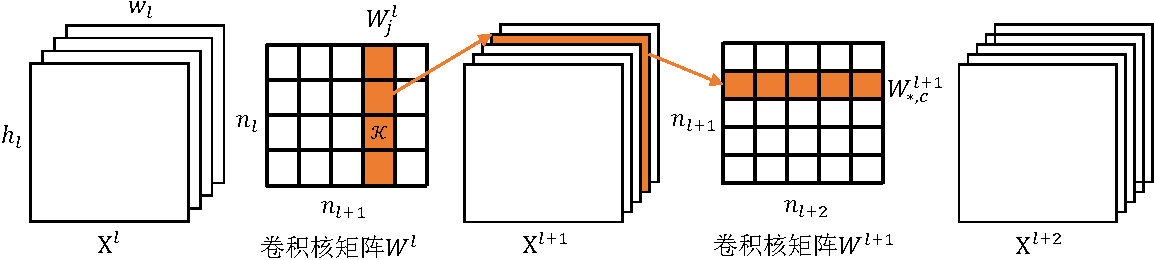
\includegraphics[clip=true, width=0.95\textwidth]{simplify.pdf}
    \caption{移除卷积核对深度卷积神经网络的影响示意图}
    \label{fig:cnn-simplify}
\end{figure}
如图~\ref{fig:cnn-simplify}所示,如果移除卷积核$W^l_j$,
则输出特征图的一个通道$X_j^{l+1}$也被移除,从而
减少$n_l k^2 h_{l+1} w_{l+1}$的运算量。由于输出通道数的减少,
下一层卷积层也可以减少一个维度的卷积核,
从而进一步进一步减少$n_{l+2}k^2h_{l+2}w_{l+2}$的运算量。

卷积神经网络的简化可以从卷积核,通道,以及卷积核内部等多个角度进行稀疏优化。本文
主要研究卷积核的结构化稀疏方法,移除整个卷积核达到减少模型参数大小,加快模型运算速度
的目的。已有算法通常采用组稀疏的方法达到结构化稀疏的目的:
\begin{equation}
    W^* = \argmin_{W} \L(X;W) \text{\quad s.t. \quad} \sum_{j=1}^{n_l}\|W_j^l\|_2^p \leq
    \lambda_l, \forall l \in [1,L]
\end{equation}
$p$取$0$时为$L_0$约束,取$1$时为$L_1$约束。组稀疏优化相对比较复杂,
$L_0$约束是非凸优化,$L_1$约束不能显示地控制卷积核的个数。
因此,本文提出了新的基于在线特征选取的深度卷积神经网络简化方法。

\subsection{基于在线特征选取的模型简化}
目前,深度网络的学习采取基于的在线优化方法,本文提出将在线组稀疏优化转化为
经典的一维在线特征选取问题,从而进行模型简化。如图~\ref{fig:cnn-simplify-w}所示,
我们在卷积层后引入辅助权重层,权重层参数是一维卷积核权重向量。
\begin{figure}[ht]
    \center
    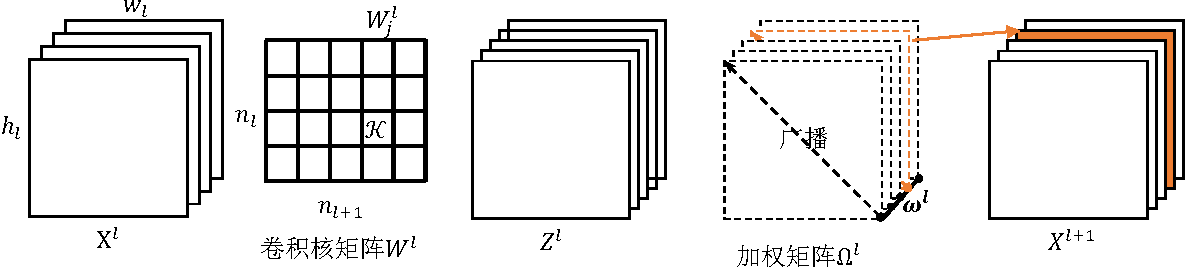
\includegraphics[clip=true, width=0.95\textwidth]{simplify-w.pdf}
    \caption{深度卷积神经网络辅助权重层模型简化}
    \label{fig:cnn-simplify-w}
\end{figure}

引入辅助权重层以后,模型简化问题的目标函数为:
\begin{eqnarray}
    W^* = \argmin_{W} \L(X;W,\bm{\omega}) \\
    \text{s.t.} \quad
    \sum_{j=1}^{n_l}(\omega_j^l)^0 \leq \lambda_l,
    -1 \leq &\omega_j^l& \leq 1,
    \forall l \in [1,L]
\end{eqnarray}
辅助权重层的前向运算为:
\begin{eqnarray}
    Z_j^l &=& \sum_{c=1}^{n_l}{W_{j,c}^l \ast X_c^l} \\
    X_j^{l+1} &=& Z_j^l \cdot \Omega_j^l \\
    \Omega_{j,:,:}^l &=& \omega_j^l
\end{eqnarray}
初始条件下所有卷积核的权重$\omega_j^l$为$1$,模型训练过程中对权重进行更新,
每次更新后利用在线特征选取算法将部分权重设为$0$,保留剩余的权重。区别与传统方法,
在线特征选取算法可以在训练过程中动态调整需要保留的卷积核,从而减小模型简化
对模型性能的影响。

区别与传统的在线特征选取算法,模型简化问题中梯度通过反向传播得到。假设反向传播到
第$l$层权重层的梯度为$G^{l+1} \in \R^{n_{l+1} \times h_{l+1} \times w_{l+1}}$,
传回第$l$层卷积层的梯度为$\nabla Z^l$,第$l$层权重层的梯度为$\nabla\bm{\omega}^l$,
权重层参数的二阶对角协方差矩阵为$\Sigma^l$,则梯度反向传播方式为:
\begin{eqnarray}
    \nabla Z^l &=& G^{l+1} \cdot \Omega^l \\
    \nabla \Omega^l &=& G^{l+1} \cdot Z^l \\
    \nabla{\omega_j}^l &=& \Sigma^l_j\sum_h\sum_w\nabla \Omega^l_{j,h,w} \\
    (\Sigma^l_j)^{-1} &=& (\Sigma^l_j)^{-1}  + \frac{\sum_h\sum_w Z^l_{j,h,w}}{\gamma}
\end{eqnarray}

\subsection{实验结果和评估}
本文在Cifar10数据集上利用VGG模型研究每一层卷积层简化对于模型准确率的影响,
实验效果如图~\ref{fig:sofs-cnn-simplify}所示。
\begin{figure}[ht]
    \center
    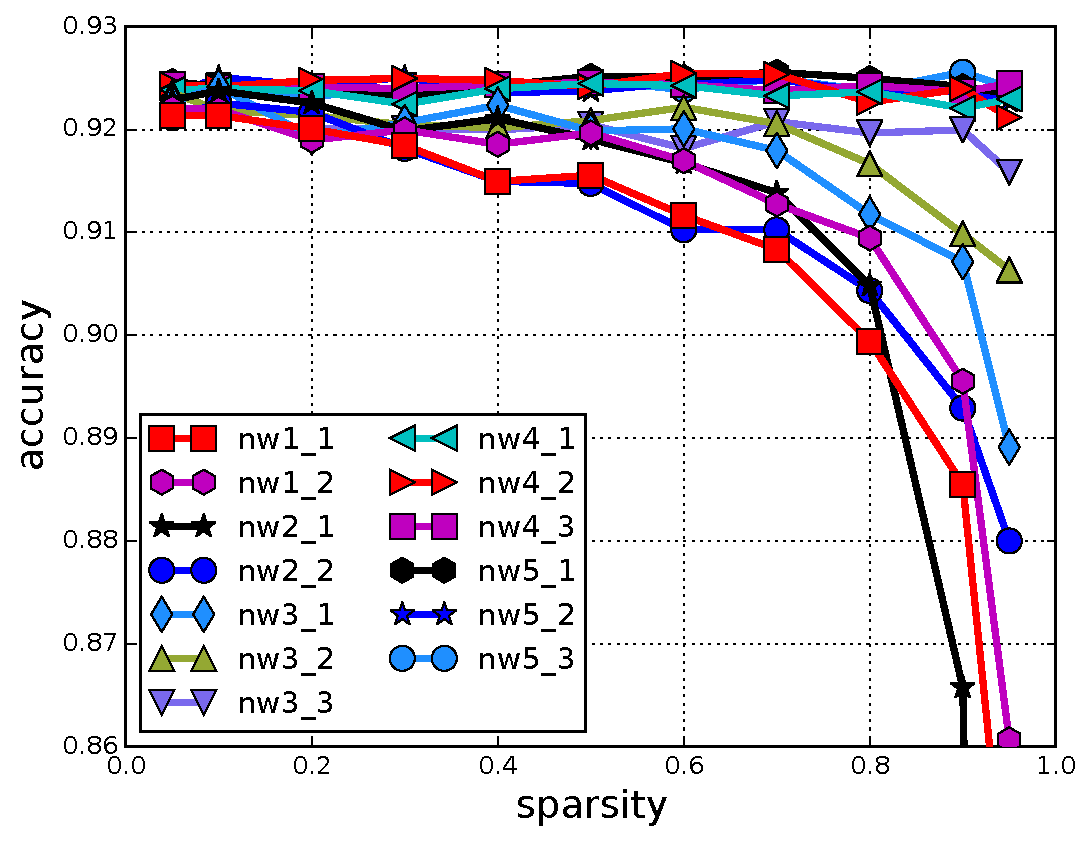
\includegraphics[clip=true, width=0.95\textwidth]{sofs-cnn-simplify.pdf}
    \caption{模型简化对模型准确率的影响}
    \label{fig:sofs-cnn-simplify}
\end{figure}

\section{小结}
本章主要解决大规模高维特征的特征选取问题,从所有特征中选取一小部分与具体问题
相关的特征。我们提出了一个新型的二阶在线特征选取算法SOFS。区别于已有的在线特征选取
算法复杂度与所有的特征维度成正比,新提出算法的复杂度被显著减少到与每个训练样本的
非零特征个数成正比。我们在中等规模和大规模的人工生成数据集和真实数据集上进行了
充分实验,比较新提出算法相对于目前最好的批处理算法和在线特征选取算法的有效性和高效性。
实验效果表明SOFS算法不仅能够达到当前最好的批处理算法相当甚至更好的测试准确率,
还可以显著减少训练的时间开销,使得SOFS算法成为处理大规模高维数据的切实可行的特征选取算法。

本章的主要贡献包括:
\begin{itemize}
    \item 我们提出了新的高效的二阶在线特征选取算法,
        用于解决大规模高维度稀疏数据的特征选取问题。
    \item 我们提出了快速一阶在线特征选取算法和二阶在线特征选取算法。尤其是二阶算法的
        复杂度从与所有维度成正比降低到与非零特征个数成正比。
    \item 我们进行了充分的实验验证了所提出的算法的有效性和高效性。
\end{itemize}

